
\section{Timing Attack}
\begin{frame}{Time analysis based attacks}{}
	\begin{quote}
		\emph{``Tor does not provide protection against end-to-end timing attacks[...]''}
	\end{quote}
	We can place a tracker after the client node and another before the server node
	and check for the connection time to profile users and nodes (and later associate IP to users.)
\end{frame}

\begin{frame}{Timing analisys based attacks}
	\begin{center}
		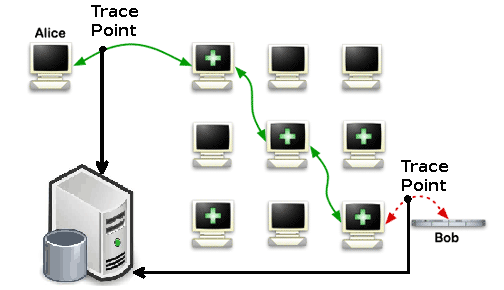
\includegraphics[scale=0.54]{imgs/timing_attack.png}
	\end{center}
\end{frame}

\begin{frame}
	\frametitle{Why simulation?}
	Simulation help us in a lot of aspects:

	\begin{itemize}
		\item Compare the performances of two onion routers (p.e. i2p vs
		Tor).
		\item To compare effects of changes in the node choice
		algorithms.
		\item \textbf{Get an idea about the timing attack feasibility 
and estimate the number of resources needed by an attacker}.
	\end{itemize}
\end{frame}

\begin{frame}{Simulation results}
	\begin{minipage}{.45\textwidth}
		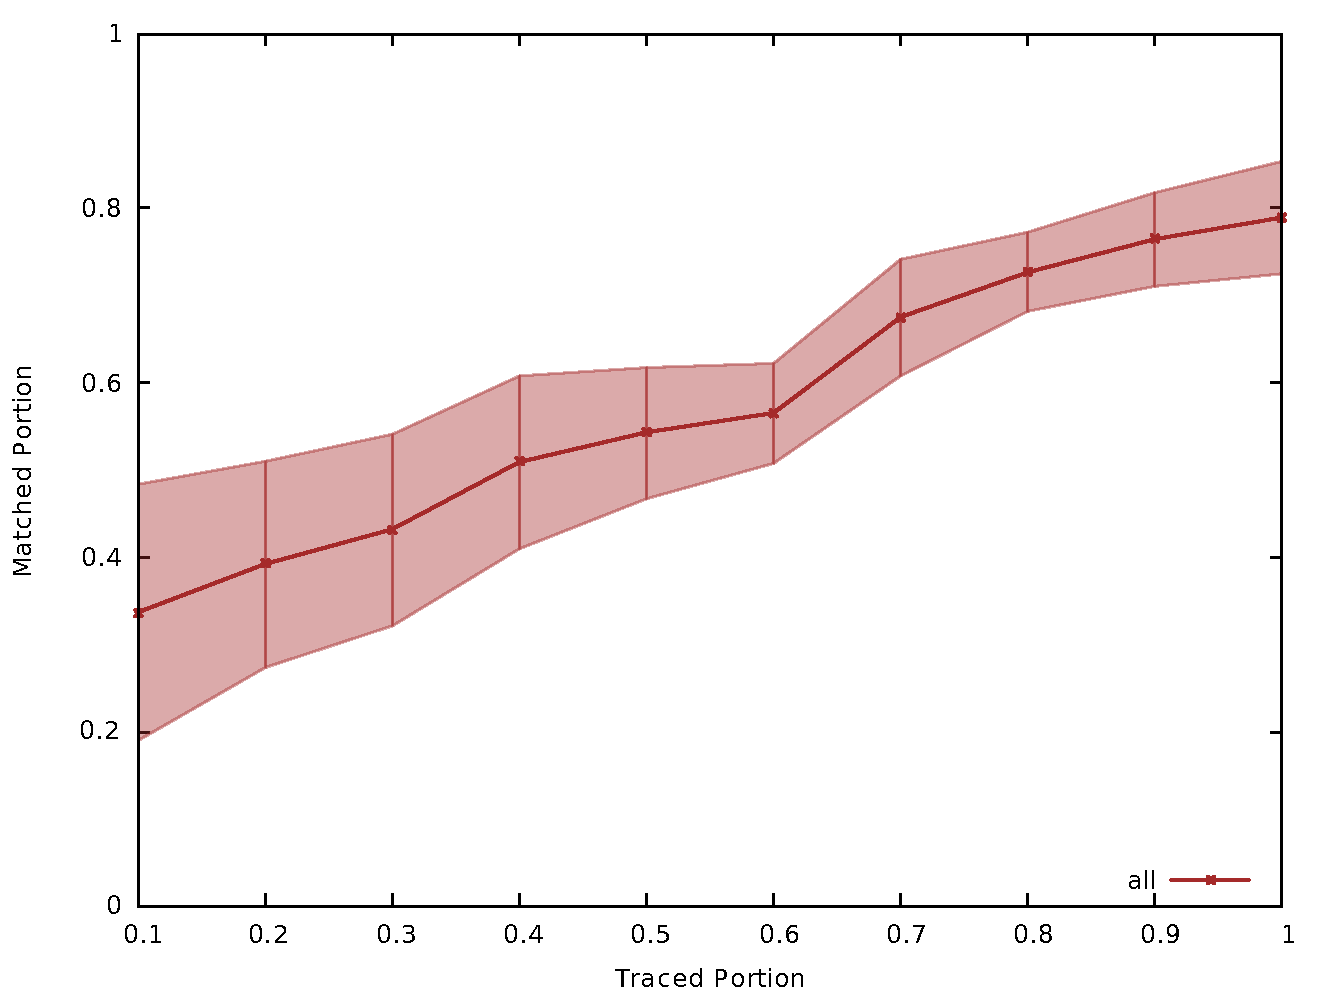
\includegraphics[scale=0.27]{imgs/cs_tport_mport.pdf}
	\end{minipage}
	\begin{minipage}{.45\textwidth}
		Tracing \textbf{half} of the Tor network, an attacker may be able to
understand the relationships between the nodes of a \textbf{quarter} of the Tor
network.
	\end{minipage}
\end{frame}

\begin{frame}{Simulation results}
	\begin{minipage}{.45\textwidth}
		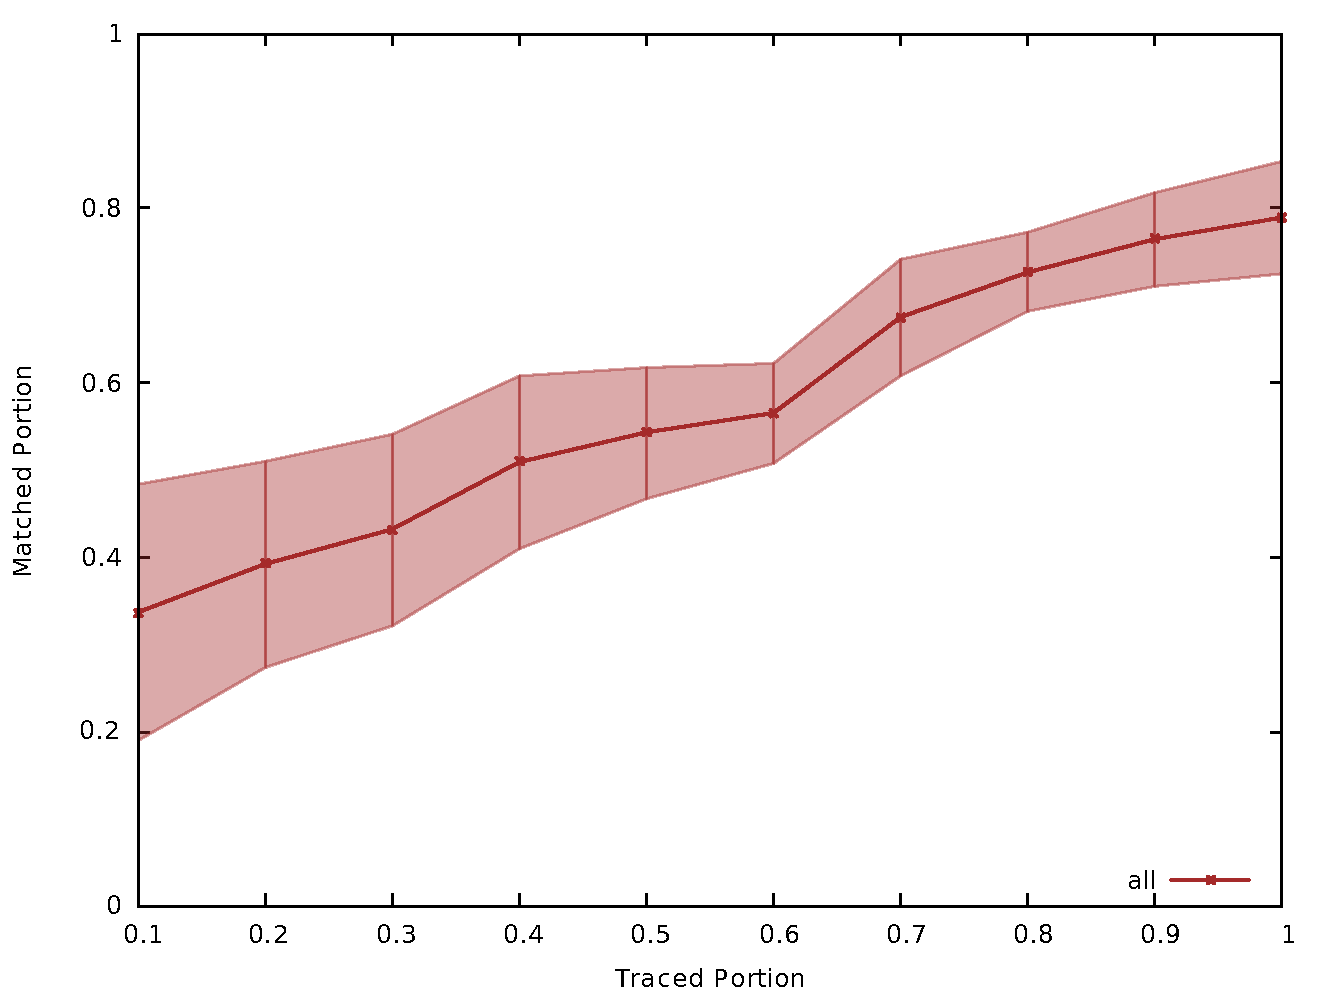
\includegraphics[scale=0.27]{imgs/cs_tport_mport.pdf}
	\end{minipage}
	\begin{minipage}{.45\textwidth}
		\begin{itemize}
			\item Timing attack is \textbf{feasible}.
			\item It requires a \textbf{LOT} of resources.
		\end{itemize}
	\end{minipage}
\end{frame}

\begin{frame}{Too much?}
	\centering
	Who can face such big amount of resources?

	\begin{figure}
		\centering
		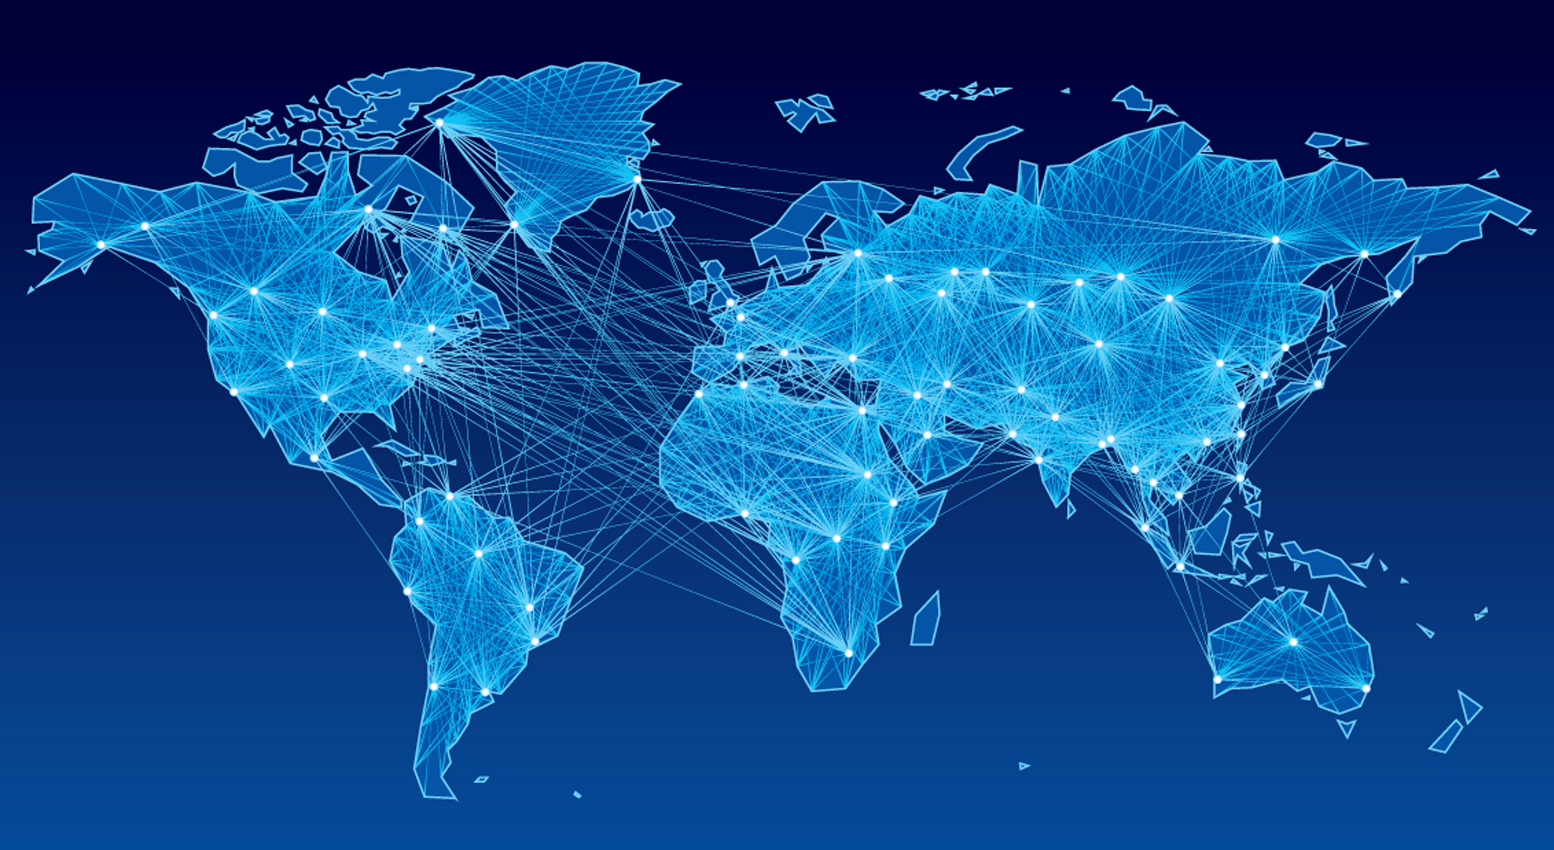
\includegraphics[scale=0.50]{imgs/bignet.jpg}
	\end{figure}

\end{frame}

\begin{frame}{NSA timing attack on clients}{NSA slides leak}
	\begin{figure}
		\centering
		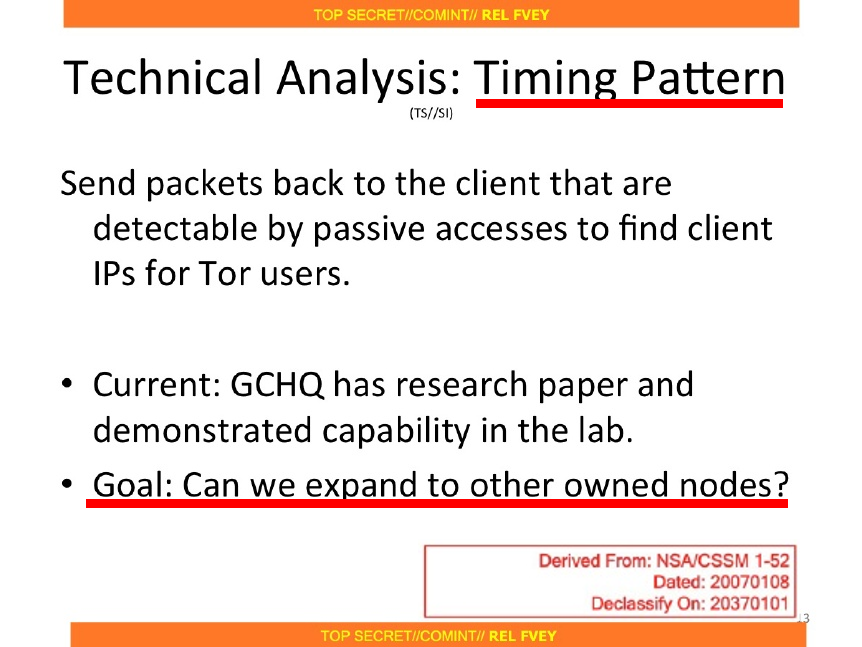
\includegraphics[scale=0.35]{imgs/nsa_timing1.png}
	\end{figure}
\end{frame}

\begin{frame}{NSA timing attack on servers}{NSA slides leak}
	\begin{figure}
		\centering
		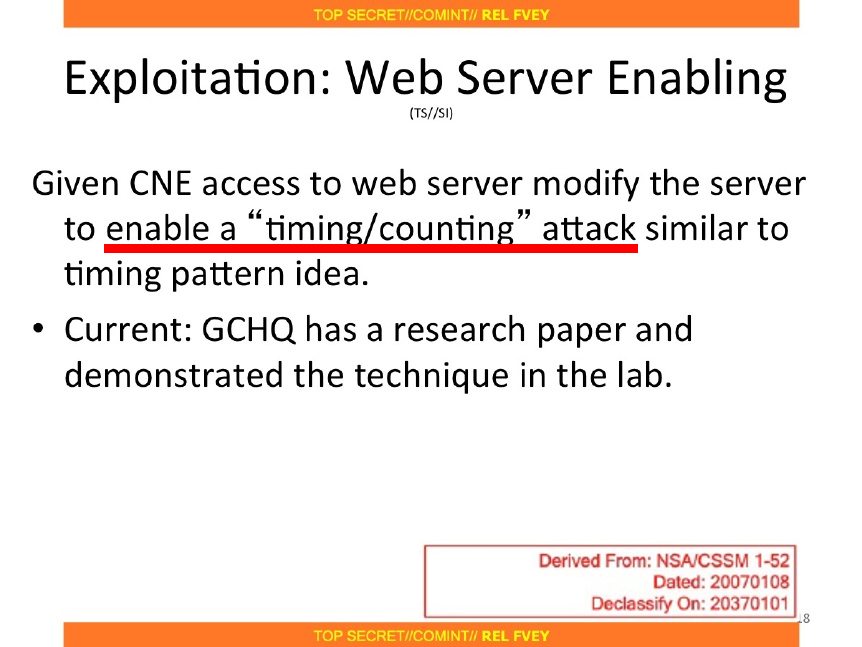
\includegraphics[scale=0.40]{imgs/nsa_timing2.png}
	\end{figure}
\end{frame}
%attacks, timing, our project -> NSA ueses timing

